\documentclass{article}
\usepackage[utf8]{inputenc}
\usepackage[T1]{fontenc}
\usepackage[provide=*]{babel}
\babelprovide[main]{polish}
\setlocalecaption{polish}{contents}{Spis treści}
\setlocalecaption{polish}{figure}{Rysunek}
\setlocalecaption{polish}{table}{Tabela}
\usepackage[a4paper, margin=2.5cm]{geometry}
\usepackage{array}
\usepackage{tocloft}
\usepackage{amsmath}
\usepackage{graphicx}
\usepackage{listings}
\usepackage{xcolor}
\usepackage{booktabs}
\usepackage{hyperref}
\usepackage{float}
\usepackage{tikz}
\usetikzlibrary{shapes, arrows, positioning, calc, shapes.geometric, backgrounds}

\tikzstyle{bpmn.start} = [circle, fill=green!30, draw=black, minimum width=12mm]
\tikzstyle{bpmn.activity} = [rectangle, fill=blue!15, draw=black, rounded corners, minimum width=15mm, minimum height=8mm]
\tikzstyle{bpmn.gateway} = [diamond, fill=yellow!30, draw=black, minimum width=12mm, aspect=2]
\tikzstyle{bpmn.event} = [circle, fill=orange!20, draw=black, minimum width=8mm]
\tikzstyle{bpmn.flow} = [->, thick, black]
\tikzstyle{bpmn.annotation} = [rectangle, fill=gray!10, draw=black, dashed, font=\footnotesize]

\definecolor{codegreen}{rgb}{0,0.6,0}
\definecolor{codegray}{rgb}{0.5,0.5,0.5}
\definecolor{codepurple}{rgb}{0.58,0,0.82}
\definecolor{backcolour}{rgb}{0.95,0.95,0.92}

\lstdefinestyle{mystyle}{
    backgroundcolor=\color{backcolour},
    commentstyle=\color{codegreen},
    keywordstyle=\color{magenta},
    numberstyle=\tiny\color{codegray},
    stringstyle=\color{codepurple},
    basicstyle=\ttfamily\footnotesize,
    breakatwhitespace=false,
    breaklines=true,
    captionpos=b,
    keepspaces=true,
    numbers=left,
    numbersep=5pt,
    showspaces=false,
    showstringspaces=false,
    showtabs=false,
    tabsize=2
}

\lstset{style=mystyle}
\renewcommand{\lstlistingname}{Kod}

\hypersetup{
    colorlinks=true,
    linkcolor=black,
    urlcolor=blue
}

\renewcommand{\cftsecleader}{\cftdotfill{\cftdotsep}}
\renewcommand{\contentsname}{Spis treści}
\renewcommand{\figurename}{Rysunek}
\renewcommand{\tablename}{Tabela}

\newcommand{\spcloudtoday}{%
    \number\day\space%
    \ifcase\month\or stycznia\or lutego\or marca\or kwietnia\or maja\or czerwca\or lipca\or sierpnia\or wrze\'snia\or pa\'zdziernika\or listopada\or grudnia\fi%
    \space\number\year%
}

\begin{document}
\title{SPCloud --- System przechowywania plików w chmurze \\
\large Dokumentacja techniczna (projekt)}
\date{\spcloudtoday}
\author{
    Imię Nazwisko 1 \\
    000000
    \and
    Imię Nazwisko 2 \\
    000000
    \and
    Imię Nazwisko 3 \\
    000000
    \and
    Imię Nazwisko 4 \\
    000000
}
\maketitle

\vfill
\begin{center}
\begin{tabular}{lr}
\toprule
\textbf{Frontend} & SvelteKit 2.x (Svelte 5), Node.js 22, TypeScript \\
\midrule
\textbf{Backend} & FastAPI, Python 3.13, SQLAlchemy (async) \\
\midrule
\textbf{Baza danych} & PostgreSQL 18 \\
\midrule
\textbf{Object Storage} & MinIO (S3-compatible) \\
\midrule
\textbf{Infrastruktura} & Docker Compose, NGINX, Raspberry Pi 5 (docelowo) \\
\bottomrule
\end{tabular}
\end{center}
\vspace{1cm}

\newpage
\tableofcontents

\newpage
\section{Wprowadzenie}

SPCloud to system przechowywania plików w chmurze umożliwiający użytkownikom przechowywanie plików w magazynie obiektowym, zarządzanie wersjami oraz pobieranie plików z poziomu aplikacji webowej. Projekt został zrealizowany jako zadanie akademickie.

Główne założenia systemu obejmują:
\begin{itemize}
    \item autentykację użytkowników oraz wymuszenie 2FA (TOTP) przy logowaniu
    \item przechowywanie plików w MinIO (S3-compatible) w modelu \textit{bucket per user}
    \item wersjonowanie plików (upload istniejącego pliku tworzy kolejną wersję)
    \item przywracanie wybranej wersji bez kopiowania obiektu w storage (zmiana \texttt{current\_version} w bazie)
    \item limit przestrzeni dyskowej per użytkownik (domyślnie 100\,MiB)
    \item możliwość oznaczania plików jako ulubione oraz pobieranie wielu plików jako ZIP
    \item logowanie zdarzeń (logowanie, operacje na plikach, pobranie logów)
\end{itemize}

Dokument opisuje architekturę systemu, kluczowe elementy implementacji oraz instrukcję uruchomienia.

\section{Zakres funkcjonalny}

\subsection{Funkcje użytkownika}
\begin{itemize}
    \item rejestracja konta i logowanie (z TOTP)
    \item konfiguracja TOTP na podstawie tokenu konfiguracyjnego (QR code)
    \item upload pliku (nowy plik lub nowa wersja)
    \item lista plików, pobieranie pliku, pobieranie wielu plików jako ZIP
    \item lista wersji pliku, pobieranie konkretnej wersji
    \item przywracanie wersji (ustawienie jako aktualnej)
    \item usuwanie pliku oraz usuwanie wersji (z wyjątkiem wersji aktualnej)
    \item oznaczanie/odznaczanie pliku jako ulubionego
    \item podgląd informacji o wykorzystaniu storage
\end{itemize}

\subsection{Funkcje administratora}
\begin{itemize}
    \item pobranie logów systemowych przez endpoint administracyjny
\end{itemize}

\section{Architektura systemu}

System jest uruchamiany kontenerowo (Docker Compose) i składa się z odseparowanych komponentów komunikujących się poprzez HTTP oraz bazę danych.

\subsection{Diagram architektury}

\begin{figure}[H]
\centering
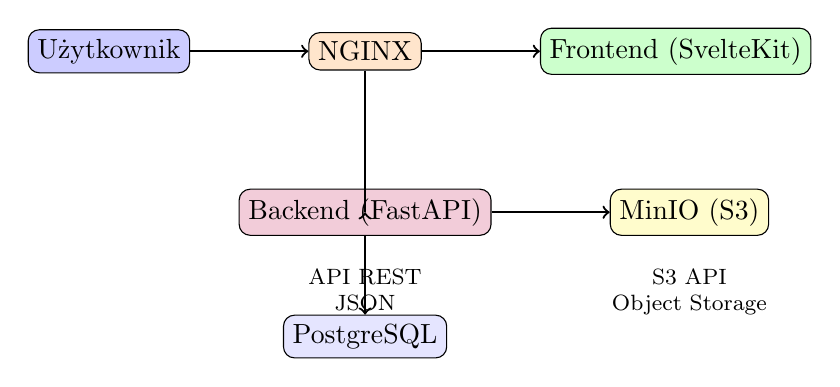
\begin{tikzpicture}[node distance=1.5cm, auto]
\node[rectangle, draw, fill=blue!20, rounded corners] (user) {Użytkownik};
\node[rectangle, draw, fill=orange!20, rounded corners, right=of user] (nginx) {NGINX};
\node[rectangle, draw, fill=green!20, rounded corners, right=of nginx] (frontend) {Frontend (SvelteKit)};
\node[rectangle, draw, fill=purple!20, rounded corners, below=of nginx] (backend) {Backend (FastAPI)};

\node[rectangle, draw, fill=blue!10, rounded corners, below=of backend, yshift=0.5cm] (db) {PostgreSQL};
\node[rectangle, draw, fill=yellow!20, rounded corners, right=of backend] (minio) {MinIO (S3)};

\draw[->, thick] (user) -- (nginx);
\draw[->, thick] (nginx) -- (frontend);
\draw[->, thick] (nginx) |- (backend);
\draw[->, thick] (backend) -- (db);
\draw[->, thick] (backend) -- (minio);

\node[below=0.3cm of backend, font=\footnotesize, align=center] {API REST\\JSON};
\node[below=0.3cm of minio, font=\footnotesize, align=center] {S3 API\\Object Storage};
\end{tikzpicture}
\caption{Architektura systemu SPCloud}
\end{figure}

Przepływ żądań przedstawia się następująco:
\begin{enumerate}
    \item Użytkownik wysyła żądanie do serwera NGINX
    \item NGINX przekierowuje ruch do odpowiedniej usługi
    \item Frontend obsługuje interfejs użytkownika
    \item Backend przetwarza logikę biznesową
    \item PostgreSQL przechowuje metadane i użytkowników
    \item MinIO przechowuje rzeczywiste pliki
\end{enumerate}

\subsection{Warstwa frontendowa}

Frontend został zbudowany z wykorzystaniem SvelteKit 2.x (Svelte 5), Node.js 22 oraz TypeScript. Główne elementy:
\begin{itemize}
    \item SvelteKit jako framework do budowy aplikacji
    \item TypeScript dla bezpieczeństwa typów
    \item komunikacja z API po HTTP (adres API przekazywany przez zmienną \texttt{PUBLIC\_API\_URL})
\end{itemize}

Komponenty frontendowe:
\begin{itemize}
    \item widoki rejestracji/logowania oraz konfiguracji TOTP
    \item przeglądarka plików (lista, ulubione, informacje o storage)
    \item upload plików oraz obsługa wersji pliku
    \item pobieranie plików (pojedynczo lub ZIP)
\end{itemize}

\subsection{Warstwa backendowa}

Backend został zaimplementowany w Pythonie z wykorzystaniem FastAPI. Wykorzystane technologie:
\begin{itemize}
    \item FastAPI jako framework webowy
    \item SQLAlchemy (async) z asyncpg dla asynchronicznej komunikacji z bazą
    \item Pydantic do walidacji danych
    \item JWT dla autentykacji
    \item Argon2id (Passlib) do hashowania haseł
    \item Python-multipart do obsługi uploadu plików
    \item Boto3 do komunikacji z MinIO (S3 API)
    \item PyOTP + qrcode do obsługi TOTP
\end{itemize}

Główne endpointy API:
\begin{itemize}
    \item \texttt{/api/v1/users/*} - rejestracja, logowanie, tokeny, dane użytkownika
    \item \texttt{/api/v1/totp/*} - konfiguracja i weryfikacja TOTP
    \item \texttt{/api/v1/files/*} - operacje na plikach oraz wersjach
    \item \texttt{/api/v1/logs/*} - pobieranie logów (admin)
\end{itemize}

\subsection{Baza danych}

System wykorzystuje PostgreSQL 18 jako relacyjną bazę danych. Schemat bazy obejmuje następujące tabele:
\begin{itemize}
    \item \texttt{users} - dane użytkowników (w tym status TOTP oraz limity storage)
    \item \texttt{files} - metadane plików (aktualna wersja, rozmiar, ulubione)
    \item \texttt{file\_versions} - historia wersji plików wraz ze ścieżką \texttt{s3://...}
    \item \texttt{refresh\_tokens} - refresh tokeny przechowywane po stronie serwera
    \item \texttt{logs} - logi zdarzeń (kto/co/kiedy)
\end{itemize}

Relacje między encjami: \texttt{users} ---\textgreater{} \texttt{files} ---\textgreater{} \texttt{file\_versions} oraz \texttt{users} ---\textgreater{} \texttt{refresh\_tokens}/\texttt{logs}.
\subsection{Object Storage}

MinIO pełni rolę kompatybilnego z S3 magazynu obiektów. Wszystkie pliki użytkowników są przechowywane w osobnych bucketach, zorganizowanych według identyfikatorów użytkowników.

Konwencje przyjęte w projekcie:
\begin{itemize}
    \item \textbf{bucket per user:} \texttt{user-\{username\}}
    \item \textbf{nazwa obiektu:} \texttt{filename\_v\{version\}.ext} (np. \texttt{dokument\_v3.txt})
    \item w bazie danych przechowywana jest ścieżka w postaci \texttt{s3://<bucket>/<key>}
\end{itemize}

Zalety wykorzystania MinIO:
\begin{itemize}
    \item Kompatybilność z API S3
    \item Wysoka wydajność przy dużych plikach
    \item Możliwość lokalnego uruchomienia
    \item Łatwa skalowalność
\end{itemize}

\section{Autentykacja i autoryzacja}

System wykorzystuje JWT (JSON Web Tokens) do autentykacji. Logowanie wymaga skonfigurowanego TOTP (2FA).

\subsection{Hasła i bezpieczeństwo}
\begin{itemize}
    \item hasła są hashowane algorytmem \textbf{Argon2id} (time\_cost=3, memory\_cost=64\,MB, parallelism=2)
    \item refresh tokeny są przechowywane w bazie danych (tabela \texttt{refresh\_tokens}); wylogowanie usuwa wszystkie refresh tokeny użytkownika
\end{itemize}

\subsection{Rodzaje tokenów}

\begin{center}
\begin{tabular}{lll}
\toprule
\textbf{Token} & \textbf{Ważność} & \textbf{Przeznaczenie} \\
\midrule
Access Token & 15 minut & Autoryzacja requestów do API \\
Refresh Token & 1 dzień & Odświeżanie access tokena \\
Setup Token (TOTP) & 15 minut & Konfiguracja TOTP po rejestracji/logowaniu \\
\bottomrule
\end{tabular}
\end{center}

\subsection{Przykładowe payloady JWT}

\begin{lstlisting}[caption={Przykładowy payload Access Token (JWT)}]
{
  "sub": "username",
  "iss": "SPCloud",
  "iat": 1736851200,
  "nbf": 1736851200,
  "exp": 1736852100,
  "jti": "abc123..."
}
\end{lstlisting}

\begin{lstlisting}[caption={Przykładowy payload Refresh Token (JWT)}]
{
  "sub": "username",
  "iss": "SPCloud",
  "iat": 1736851200,
  "nbf": 1736851200,
  "exp": 1736937600,
  "jti": "xyz789...",
  "type": "refresh"
}
\end{lstlisting}

\begin{lstlisting}[caption={Przykładowy payload Setup Token (TOTP)}]
{
  "sub": "username",
  "exp": 1736852100,
  "type": "totp_setup"
}
\end{lstlisting}

\subsection{Flow rejestracji i logowania (TOTP)}

Po rejestracji oraz przy pierwszym logowaniu użytkownik otrzymuje \textbf{Setup Token} do konfiguracji TOTP.
Po skonfigurowaniu aplikacji uwierzytelniającej (np. Google Authenticator) użytkownik loguje się już zawsze z kodem TOTP.

\begin{lstlisting}[caption={Schemat rejestracji/logowania (uproszczony)}]
POST /api/v1/users/register  ->  Setup Token (TOTP, 15 min)
POST /api/v1/totp/setup      ->  QR Code + secret (wymaga Setup Token)
POST /api/v1/totp/verify     ->  Access + Refresh Token (wymaga Setup Token)

POST /api/v1/users/login     ->  jesli TOTP nie skonfigurowany: Setup Token
                              jesli TOTP skonfigurowany: 403 "TOTP verification required"
POST /api/v1/users/login/totp -> Access + Refresh Token
\end{lstlisting}

\section{Wersjonowanie plików}

System automatycznie tworzy wersje plików przy każdej zmianie, umożliwiając przywracanie wcześniejszych stanów.

\subsection{Wersjonowanie: zasady działania}

\begin{figure}[H]
\centering
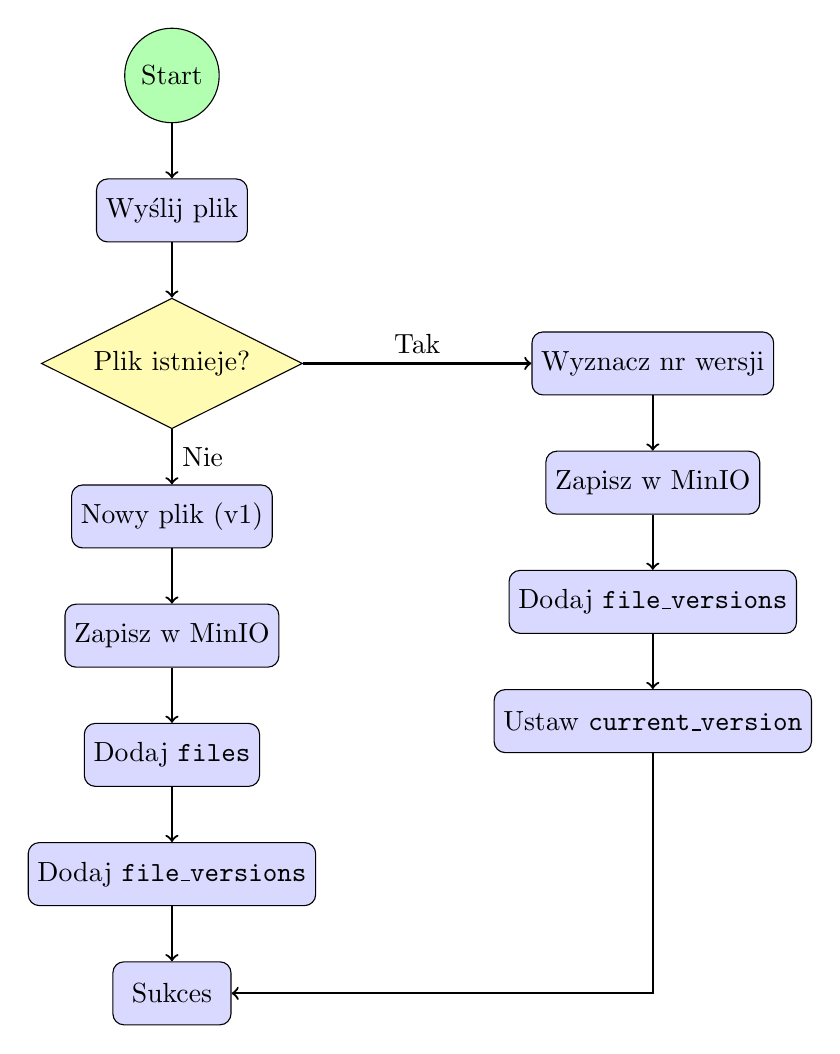
\begin{tikzpicture}[node distance=0.7cm]
\node[bpmn.start] (start) {Start};
\node[bpmn.activity, below=of start] (upload) {Wyślij plik};
\node[bpmn.gateway, below=of upload] (exists) {Plik istnieje?};
\node[bpmn.activity, right=of exists, xshift=2.2cm] (nextver) {Wyznacz nr wersji};
\node[bpmn.activity, below=of nextver] (save_minio_existing) {Zapisz w MinIO};
\node[bpmn.activity, below=of save_minio_existing] (insert_version) {Dodaj \texttt{file\_versions}};
\node[bpmn.activity, below=of insert_version] (set_current) {Ustaw \texttt{current\_version}};

\node[bpmn.activity, below=of exists] (new) {Nowy plik (v1)};
\node[bpmn.activity, below=of new] (save_minio_new) {Zapisz w MinIO};
\node[bpmn.activity, below=of save_minio_new] (insert_file) {Dodaj \texttt{files}};
\node[bpmn.activity, below=of insert_file] (insert_version_new) {Dodaj \texttt{file\_versions}};

\node[bpmn.activity, below=of insert_version_new] (success) {Sukces};

\draw[bpmn.flow] (start) -- (upload);
\draw[bpmn.flow] (upload) -- (exists);
\draw[bpmn.flow] (exists) -- node[above] {Tak} (nextver);
\draw[bpmn.flow] (nextver) -- (save_minio_existing);
\draw[bpmn.flow] (save_minio_existing) -- (insert_version);
\draw[bpmn.flow] (insert_version) -- (set_current);
\draw[bpmn.flow] (set_current) |- (success);

\draw[bpmn.flow] (exists) -- node[right] {Nie} (new);
\draw[bpmn.flow] (new) -- (save_minio_new);
\draw[bpmn.flow] (save_minio_new) -- (insert_file);
\draw[bpmn.flow] (insert_file) -- (insert_version_new);
\draw[bpmn.flow] (insert_version_new) -- (success);
\end{tikzpicture}
\caption{Diagram BPMN - Wersjonowanie plików}
\end{figure}

Mechanizm wersjonowania działa następująco:
\begin{enumerate}
    \item Przesłany plik jest weryfikowany pod kątem istnienia
    \item Jeśli plik istnieje (ta sama nazwa w obrębie użytkownika), tworzona jest nowa wersja \texttt{vN+1}
    \item Obiekt w MinIO jest zapisywany pod nazwą \texttt{filename\_v\{n\}.ext}
    \item W bazie danych aktualizowane są metadane i pole \texttt{current\_version}
\end{enumerate}

\noindent Przywracanie wersji nie kopiuje danych w MinIO --- system jedynie zmienia \texttt{current\_version} w tabeli \texttt{files}.

\subsection{Model danych plików}

\begin{lstlisting}[language=SQL, caption={Fragment schematu bazy danych (plik + wersje)}]
files (
  id UUID PK,
  name TEXT,
  owner TEXT FK -> users.username,
  current_version INT,
  size INT,
  is_favorite BOOL,
  created_at TIMESTAMPTZ,
  updated_at TIMESTAMPTZ,
  UNIQUE(owner, name)
)

file_versions (
  id UUID PK,
  file_id UUID FK -> files.id,
  version_number INT,
  path TEXT,
  size INT,
  created_at TIMESTAMPTZ,
  created_by TEXT FK -> users.username
)
\end{lstlisting}

\section{Endpointy API}

Wszystkie endpointy FastAPI są wystawione pod prefiksem \texttt{/api/v1}. Autoryzacja odbywa się przez nagłówek \texttt{Authorization: Bearer <token>}.

\subsection{Użytkownicy (users)}

\begin{center}
\begin{tabular}{p{1.6cm}p{5.4cm}p{8.0cm}}
\toprule
\textbf{Metoda} & \textbf{Endpoint} & \textbf{Opis} \\
\midrule
POST & \texttt{/users/register} & Rejestracja (zwraca Setup Token do TOTP) \\
POST & \texttt{/users/login} & Logowanie (Setup Token jeśli TOTP nie skonfigurowany, w przeciwnym razie 403) \\
POST & \texttt{/users/login/totp} & Logowanie z kodem TOTP (zwraca Access+Refresh) \\
POST & \texttt{/users/refresh} & Odświeżenie Access Tokenu na podstawie Refresh Tokenu \\
POST & \texttt{/users/logout} & Wylogowanie (usuwa refresh tokeny użytkownika) \\
GET & \texttt{/users/me} & Dane użytkownika + limity storage + status TOTP \\
GET & \texttt{/users/isadmin} & Informacja czy użytkownik ma rolę \texttt{admin} \\
\bottomrule
\end{tabular}
\end{center}

\subsection{TOTP}

Endpointy \texttt{/totp/setup} oraz \texttt{/totp/verify} wymagają \textbf{Setup Token} (token typu \texttt{totp\_setup}).

\begin{center}
\begin{tabular}{p{1.6cm}p{5.4cm}p{8.0cm}}
\toprule
\textbf{Metoda} & \textbf{Endpoint} & \textbf{Opis} \\
\midrule
POST & \texttt{/totp/setup} & Generuje sekret oraz QR Code do konfiguracji aplikacji TOTP \\
POST & \texttt{/totp/verify} & Weryfikuje kod TOTP i zwraca Access+Refresh Token \\
GET & \texttt{/totp/status} & Zwraca status konfiguracji TOTP dla użytkownika \\
\bottomrule
\end{tabular}
\end{center}

\subsection{Pliki (files)}

\begin{center}
\begin{tabular}{p{1.6cm}p{5.4cm}p{8.0cm}}
\toprule
\textbf{Metoda} & \textbf{Endpoint} & \textbf{Opis} \\
\midrule
POST & \texttt{/files/upload} & Upload pliku (nowy plik lub nowa wersja) \\
GET & \texttt{/files/} & Lista plików użytkownika \\
GET & \texttt{/files/me} & Informacje o wykorzystaniu storage i statystyki \\
GET & \texttt{/files/download/\{id\}} & Pobranie aktualnej wersji pliku \\
POST & \texttt{/files/download} & Pobranie wielu plików jako ZIP \\
DELETE & \texttt{/files/\{id\}} & Usunięcie pliku (wszystkie wersje) \\
POST & \texttt{/files/change-is-favorite} & Oznaczenie/odznaczenie pliku jako ulubiony \\
GET & \texttt{/files/\{id\}/versions} & Lista wersji pliku \\
GET & \texttt{/files/\{id\}/versions/\{n\}} & Pobranie konkretnej wersji \texttt{n} \\
POST & \texttt{/files/\{id\}/restore/\{n\}} & Przywrócenie wersji \texttt{n} (zmiana \texttt{current\_version}) \\
DELETE & \texttt{/files/\{id\}/versions/\{n\}} & Usunięcie wersji \texttt{n} (nie można usunąć aktualnej) \\
\bottomrule
\end{tabular}
\end{center}

\subsection{Logi (admin)}

\begin{center}
\begin{tabular}{p{1.6cm}p{5.4cm}p{8.0cm}}
\toprule
\textbf{Metoda} & \textbf{Endpoint} & \textbf{Opis} \\
\midrule
GET & \texttt{/logs/download/\{limit\}} & Pobranie ostatnich \texttt{limit} logów (wymaga roli \texttt{admin}) \\
\bottomrule
\end{tabular}
\end{center}

\section{Logowanie zdarzeń}

Każda istotna akcja jest logowana do tabeli \texttt{logs}. Log zawiera m.in. timestamp (UTC), nazwę użytkownika, akcję, status (SUCCESS/FAILED), opcjonalnie \texttt{file\_id} oraz pole \texttt{details} (JSON jako string, np. IP klienta).

\begin{lstlisting}[caption={Lista kluczowych typów akcji logowanych w systemie}]
LOGIN, LOGOUT, REGISTER,
FILE_UPLOAD, FILE_DOWNLOAD, FILE_MANY_DOWNLOAD, FILE_DELETE,
FILE_FAVORITE, FILE_UNFAVORITE,
FILE_VERSION_CREATE, FILE_VERSION_RESTORE, FILE_VERSION_DELETE,
LOG_DOWNLOAD
\end{lstlisting}

\section{Instalacja i uruchomienie}

System może być uruchomiony w środowisku lokalnym lub na serwerze produkcyjnym.

\subsection{Wymagania}
\begin{itemize}
    \item Docker Engine 24.x
    \item Docker Compose V2
    \item Minimum 4GB RAM
    \item 20GB wolnego miejsca na dysku
\end{itemize}

\subsection{Konfiguracja}

Zmienne środowiskowe konfigurowane są poprzez plik \texttt{.env}. Najważniejsze zmienne backendu:

\begin{center}
\begin{tabular}{ll}
\toprule
\textbf{Zmienna} & \textbf{Opis} \\
\midrule
DB\_URL & Connection string do PostgreSQL (SQLAlchemy async) \\
JWT\_SECRET & Sekret do podpisu JWT \\
JWT\_EXPIRE\_MIN & Czas życia Access Tokenu (minuty) \\
JWT\_REFRESH\_EXPIRE\_DAYS & Czas życia Refresh Tokenu (dni) \\
JWT\_ISSUER & Issuer w JWT \\
MINIO\_ENDPOINT & Adres serwera MinIO (np. \texttt{minio:9000}) \\
MINIO\_ACCESS\_KEY & Klucz dostępu MinIO \\
MINIO\_SECRET\_KEY & Sekret dostępu MinIO \\
MINIO\_SECURE & Czy używać SSL do MinIO (true/false) \\
\bottomrule
\end{tabular}
\end{center}

\subsection{Uruchomienie}

\begin{enumerate}
    \item Sklonuj repozytorium
    \item Skonfiguruj plik \texttt{.env}
    \item Uruchom kontenery: \texttt{docker compose up -d --build}
    \item Backend inicjalizuje strukturę bazy danych przy starcie aplikacji
    \item Otwórz przeglądarkę pod adresem \texttt{https://localhost} (frontend)
\end{enumerate}

\subsection{Porty i routing}

\begin{itemize}
    \item \textbf{NGINX:} \texttt{80} (redirect do HTTPS) oraz \texttt{443} (reverse proxy)
    \item \textbf{Frontend:} domyślnie \texttt{3000} (kontener) oraz port hosta \texttt{\$FRONTEND\_PORT} (domyślnie 3000)
    \item \textbf{Backend:} \texttt{8000}
    \item \textbf{MinIO:} \texttt{9000} (S3 API) oraz \texttt{9001} (konsola)
    \item \textbf{PostgreSQL:} \texttt{5432} w sieci kontenerów oraz port hosta \texttt{\$POSTGRES\_PORT}
\end{itemize}

NGINX przekazuje ruch do backendu dla ścieżek \texttt{/api/*} oraz do frontendu dla pozostałych ścieżek.

\subsection{Infrastruktura produkcyjna}

Środowisko produkcyjne zostało uruchomione na Raspberry Pi 5 z następującą konfiguracją:
\begin{itemize}
    \item System: Ubuntu Server 24.04 LTS
    \item Docker z wtyczką Compose
    \item NGINX jako reverse proxy
    \item Certyfikaty Let's Encrypt dla HTTPS
\end{itemize}

\section{Podsumowanie}

SPCloud to system przechowywania plików w chmurze z autentykacją dwuskładnikową (TOTP), wersjonowaniem plików oraz separacją danych w magazynie obiektowym (bucket per user). System został uruchomiony w architekturze kontenerowej (Docker Compose) z reverse proxy NGINX.

Potencjalne kierunki rozwoju:
\begin{itemize}
    \item dodanie szyfrowania plików po stronie klienta
    \item rozbudowa o role/uprawnienia oraz panel administracyjny
    \item dodanie mechanizmu udostępniania plików (linki czasowe)
    \item usprawnienie obsługi bardzo dużych plików (np. multipart upload)
\end{itemize}

\end{document}
